% !Mode:: "TeX:UTF-8"
\documentclass[QAofGroup.tex]{subfiles}
\begin{filecontents*}{blood.tex}
\documentclass{standalone}
\usepackage{ctex}
\usepackage{tikz}
\begin{document}
	\definecolor{blood}{RGB}{220,48,35}
	\definecolor{plasma}{RGB}{250,255,114}
	\definecolor{erythrocyte}{RGB}{190,0,47}
	\begin{tikzpicture}
	\begin{scope}
	\draw[thick](-0.5,0) rectangle(0.5,11);
	\draw[thick](-0.5,0)--++(-0.5,-0.1)--++(0,-0.05)--++(2,0) --++(0,0.05)--++(-0.5,0.1);
	\fill[color=blood](-0.46,0.04) rectangle(0.46,10);
	\fill[color=blood](-0.46,10)--(-0.46,10.1) parabola[parabola height=-1mm](0.46,10.1)--(0.46,10)--cycle;
	\foreach \x in{1,2,...,10}
	{\foreach \y in{1,2,...,9}
		\draw (0.5,\x-0.1*\y)--++(-0.2,0);
		\draw (0.5,\x)--++(-0.3,0) node [left]{\scriptsize\x};}
	\end{scope}
	\draw[<->,thin](-1.5,0)--(-1.5,10) node[midway, fill=white] {\small 全血};
	\draw[ultra thin](-1.0,10)--(-1.7,10);
	\draw[ultra thin](-1.0,0)--(-1.7,0);
	\begin{scope}[xshift=3cm]
	\draw[thick](-0.5,0)rectangle(0.5,11);
	\draw[thick](-0.5,0)--++(-0.5,-0.1)--++(0,-0.05)--++(2,0) --++(0,0.05)--++(-0.5,0.1);
	\fill[color=erythrocyte](-0.46,0.04) rectangle(0.46,4.5);
	\fill[color=plasma](-0.46,5) rectangle(0.46,10);
	\fill[color=plasma](-0.46,10)--(-0.46,10.1) parabola[parabola height=-1mm](0.46,10.1) --(0.46,10)--cycle;
	\foreach \x in{1,2,...,10}
	{\foreach \y in{1,2,...,9}
		\draw (0.5,\x-0.1*\y)--++(-0.2,0);
		\draw (0.5,\x)--++(-0.3,0) node [left]{\scriptsize\x};}
	\end{scope}
	
	\draw[<->,thin](4.5,5)--(4.5,10) node[midway, fill=white] {\small 血浆};
	\draw[ultra thin](4.0,10)--(4.7,10);
	\draw[ultra thin](4.0,5)--(4.7,5);
	\draw[ultra thin](4.0,4.5)--(4.7,4.5);
	\draw[ultra thin](4.0,0)--(4.7,0);
	\draw[<->,thin](4.5,0)--(4.5,4.5) node[midway, fill=white] {\small 红细胞};
	\draw[>=stealth,<-](4.1,4.75)--(4.5,4.75) node [right] {\small 白细胞和血小板};
	\end{tikzpicture}
\end{document}
\end{filecontents*}

\begin{document}
%-=-=-=-=-=-=-=-=-=-=-=-=-=-=-=-=-=-=-=-=-=-=-=-=
%
%	CHAPTER
%
%-=-=-=-=-=-=-=-=-=-=-=-=-=-=-=-=-=-=-=-=-=-=-=-=

%%================================================================
\chapter{20180405}\label{ch180404}
%----------------------------------------------------------------------------------------
\begin{qst}\label{Q2018040501}
	如何安装自己定义的宏包?\index{安装宏包}
\end{qst}
\ans 最简单的使用可以放在当前TeX文档所在文件夹,如果要安装,个人包建议放在 personal texmf tree 而不是系统自带的texmf tree。参考这个网页。\href{https://tex.stackexchange.com/questions/1137/where-do-i-place-my-own-sty-or-cls-files-to-make-them-available-to-all-my-te/1138#1138}{Where do I place my own .sty or .cls files, to make them available to all my .tex files?}

\begin{qst}\label{Q2018040502}
 如何绘制采血试管?\index{试管图}
\end{qst}
\ans 可以使用Tikz直接绘制。
\inputminted[fontsize=\normalsize,linenos,breaklines]{tex}{blood.tex}
    \ifcompile\immediate\write18{xelatex blood.tex}\fi
\begin{center}
	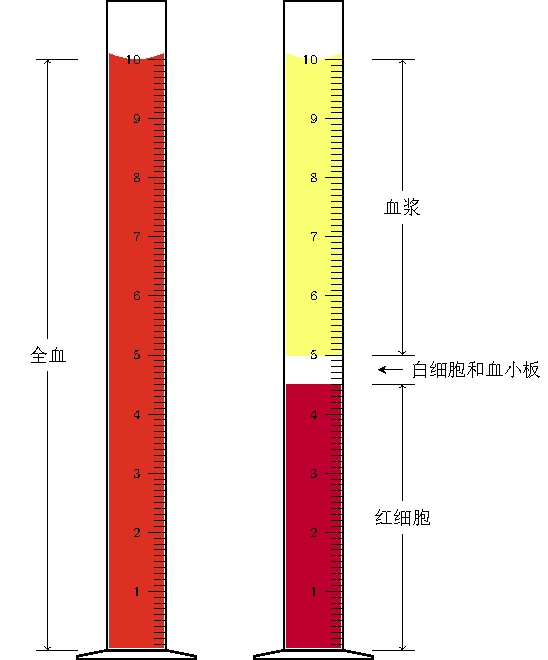
\includegraphics[width = 0.75\linewidth]{blood.pdf}
\end{center}


\end{document} 